\section{Part 1A: Vowel Formant Analysis}

In this part, you will analyze recordings of speakers of American English uttering the following words:

\begin{enumerate}
\item heed -- [h i\textlengthmark{} d]
\item hid -- [h \textsci{} d]
\item head -- [h \textepsilon{} d] 
\item had -- [h \ae {} d]
\item hod -- [h \textscripta\textlengthmark{} d]
\item hawed -- [h \textopeno\textlengthmark{} d]
\item hood -- [h \textupsilon{} d]
\item who'd -- [h u\textlengthmark{} d]
\end{enumerate}

You should repeat each word approximately 5 times. Save each repetition in a different file, then get the vowel formants (F1, F2 and F3) values as given by \Praat{} and store them in a spreadsheet program --- \MSExcel{} or \OpOff{} are fine. Remember to label each column and line so you know what the values refer to.

Once you have measured all the formant values of your recordings, you should average the values of the formants for each vowel and then plot those in a F1-F2 graph (F1 as the y--axis and F2 as the x--axis).


\subsubsection{Looking at the spectrogram}

Once you have saved the recording, you should be able to see it on your object list (figure~\ref{step1look}).

\begin{figure}[!tbp]
\caption{\Praat{} -- Object in List}
\label{step1look}
	\begin{center}
		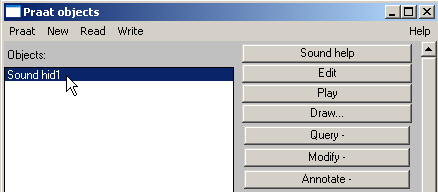
\includegraphics[width=0.8\textwidth]{./figures/PraatObjectinList}
	\end{center}
\end{figure}


Now you can do a lot of things to it. Since this lab is about making acoustic measurements, you should click on the \softmenu{Edit} button (figure~\ref{step2look}).

\begin{figure}[!tbp]
\caption{\Praat{} -- How to display the Spectrogram}
\label{step2look}
	\begin{center}
		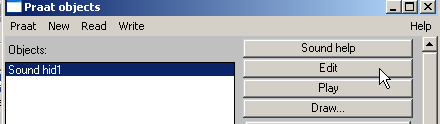
\includegraphics[width=0.8\textwidth]{./figures/PraatEditButton}
	\end{center}
\end{figure}

This will open a window where you can see both the waveform and its spectrogram (figure~\ref{step3look}). If you can't see the spectrogram, go to \softmenu{Spectrum} $>$ \softmenu{Show Spectrogram}.

In case your spectrogram is not as clear as the one we saw in class or as the one I show here (figure~\ref{step3look}), you can try the following:

\begin{enumerate}
\item Record again
\item ``Prettify'' the spectrogram a little bit. Go to \softmenu{Spectrum} $>$ \softmenu{Spectrogram settings}. Look for the \softmenu{Dynamic Range} (dB) field (figure~\ref{step4look}). The default value is 50. Try lowering it in 3dB decrements and see what it does to your spectrogram. Can you see your formants a little better? Compare figures~\ref{step3look} and~\ref{step5look}.
\end{enumerate}


\begin{figure}[!tbp]
\caption{\Praat{} -- Edit Window}
\label{step3look}
	\begin{center}
		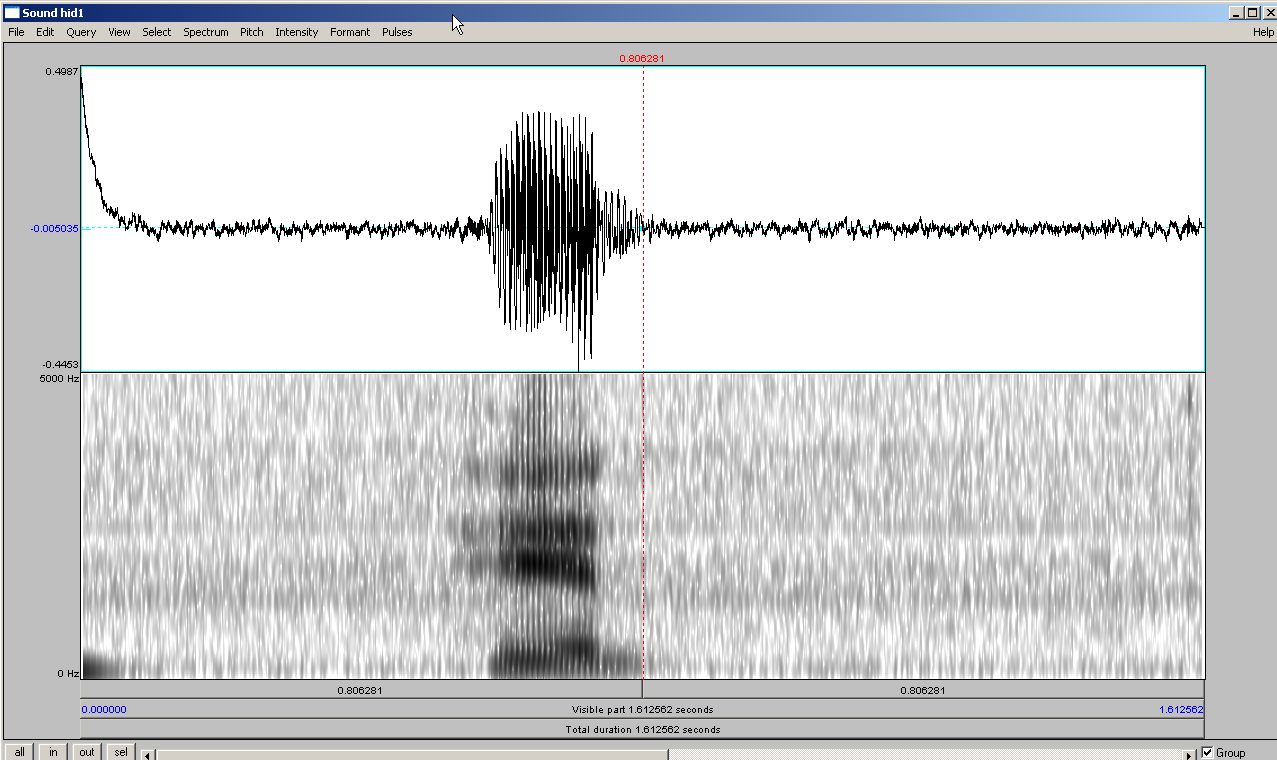
\includegraphics[width=0.8\textwidth]{./figures/PraatEditWindow}
	\end{center}
\end{figure}

\begin{figure}[!tbp]
\caption{\Praat{} -- Changing the value of Dynamic Range}
\label{step4look}
	\begin{center}
		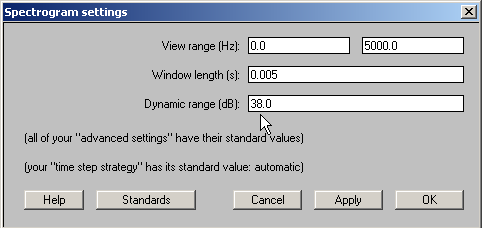
\includegraphics[width=0.8\textwidth]{./figures/PraatEditWindowSpectroSettingsDynRange}
	\end{center}
\end{figure}

\begin{figure}[!tbp]
\caption{\Praat{} -- Edit Window with modified Dynamic Range value (38dB)}
\label{step5look}
	\begin{center}
		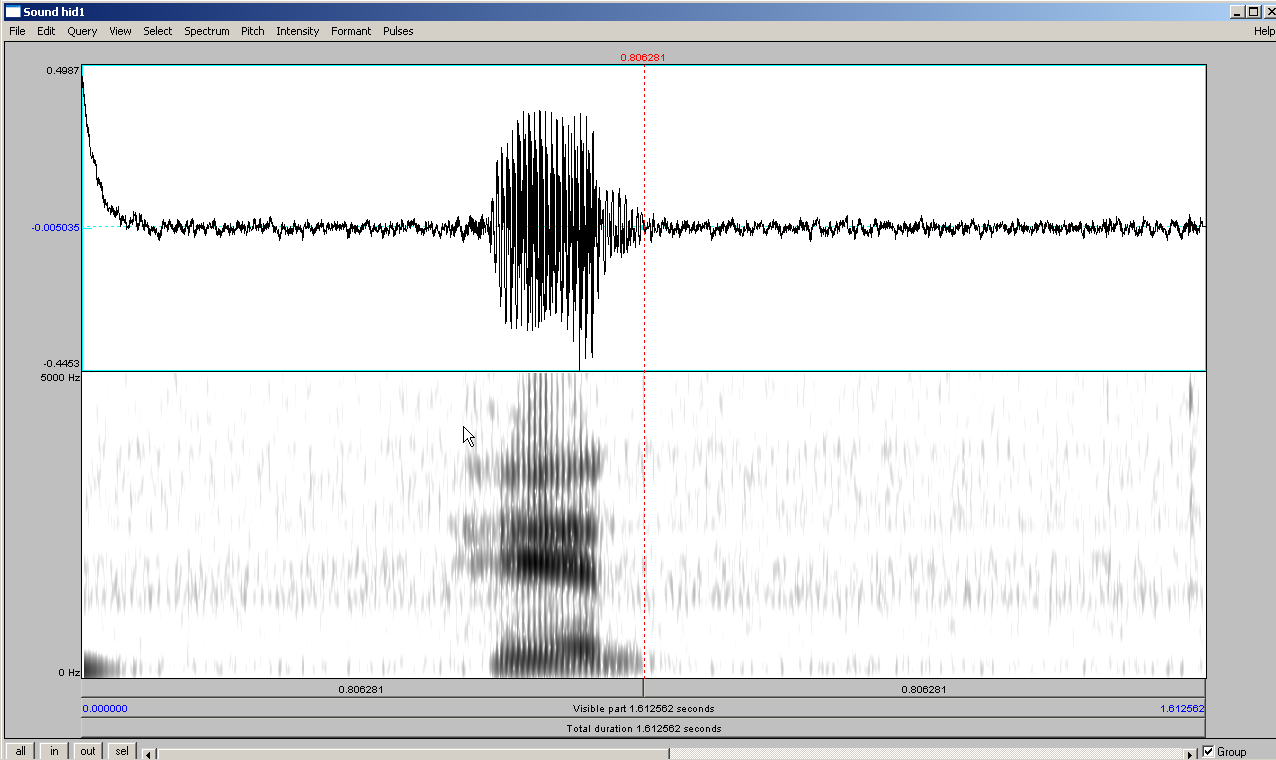
\includegraphics[width=0.8\textwidth]{./figures/PraatEditWindowPretty41dB}
	\end{center}
\end{figure}

\subsection{Making the measurements}

Once you have your spectrogram in front of you, go to \softmenu{Formant} $>$ \softmenu{Show Formants}. You should see the formants with a bunch of red dots overlaid (figure~\ref{step1measure})

\begin{figure}[!tbp]
\caption{\Praat{} -- Formant tracking}
\label{step1measure}
	\begin{center}
		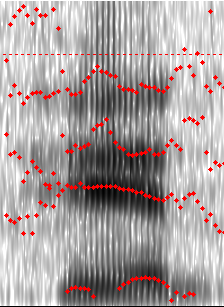
\includegraphics[width=0.8\textwidth]{./figures/PraatFormantTrack}
	\end{center}
\end{figure}

As you can see, \Praat{}'s formant tracking algorithm is pretty neat, but it is not flawless. Notice the gap in F1 and the bump in F3 (figure~\ref{step1measure})?

\begin{figure}[!tbp]
\caption{\Praat{} -- Selecting the window of interest for the measurement of the Formants}
\label{step2measure}
	\begin{center}
		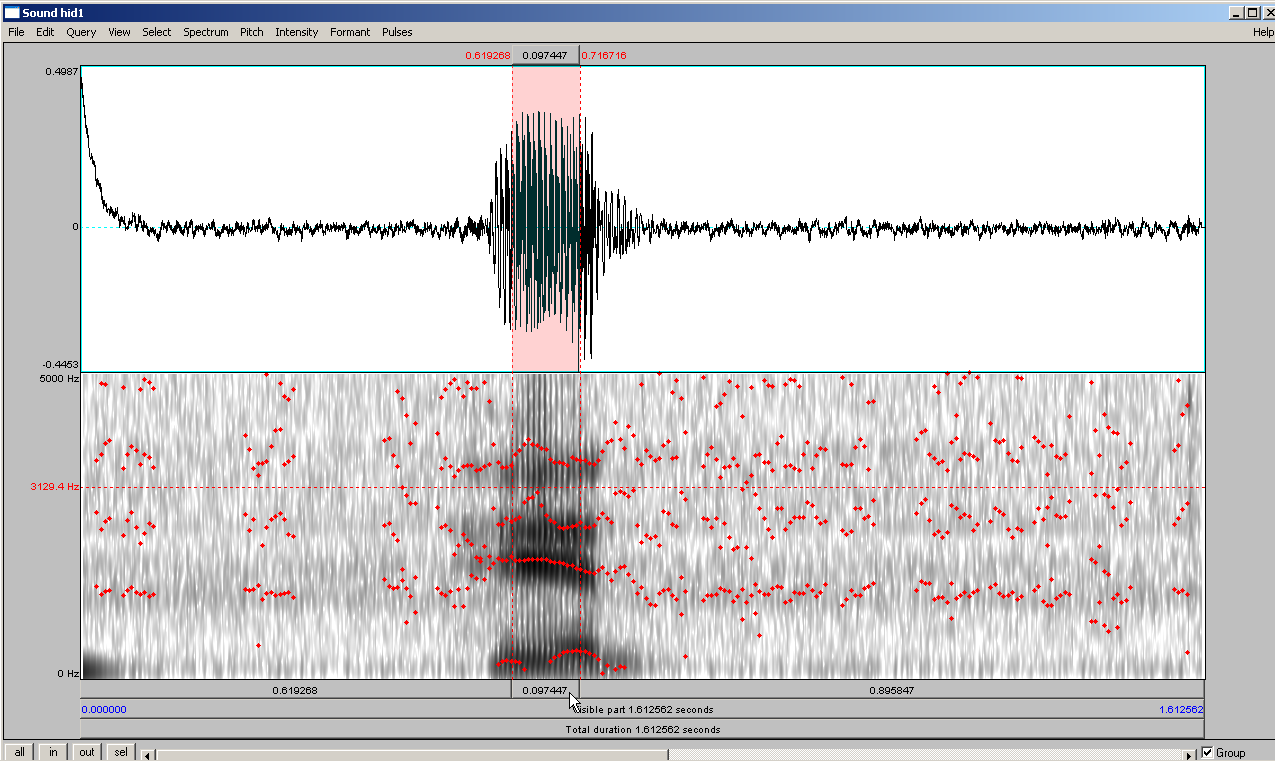
\includegraphics[width=0.8\textwidth]{./figures/PraatSpectrogrSelection}
	\end{center}
\end{figure}

If \Praat{} gave you reasonable formant tracks, then you can select a window over the center of the vowel (figure~\ref{step2measure}) --- a tip: to play the selection, click where the mouse cursor is on figure~\ref{step2measure} --- and go to \softmenu{Get first formant} (figure~\ref{step3measure}). This should give you a window with a value. Notice what the value actually is.

\begin{figure}[!tbp]
\caption{\Praat{} -- Getting the Formants automatically}
\label{step3measure}
	\begin{center}
		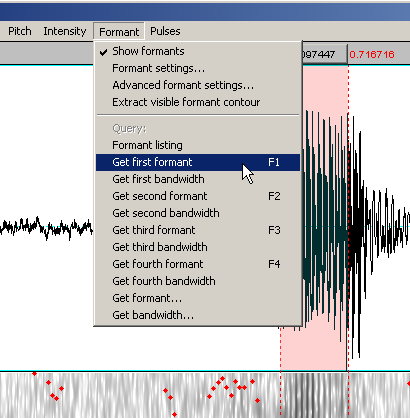
\includegraphics[width=0.8\textwidth]{./figures/PraatSpectrogrGetF1}
	\end{center}
\end{figure}


If \Praat{} gave you formant tracks that don't seem to capture the formants you see adequately, then you can try to pin a couple of points in the formants, get their values, average them and record that value in the spreadsheet. To get the value of any particular point, you can just click on it and \Praat{} will give you its value on the left side of the spectrogram (figure~\ref{step4measure}). You can then jot down the numbers somewhere. If you want numbers that you can copy and paste, just click on the point, and then go to \softmenu{Spectrum} $>$ \softmenu{Get frequency at cursor} (figure~\ref{step5measure}).

\begin{figure}[!tbp]
\caption{\Praat{} -- Getting the Formants with the mouse}
\label{step4measure}
	\begin{center}
		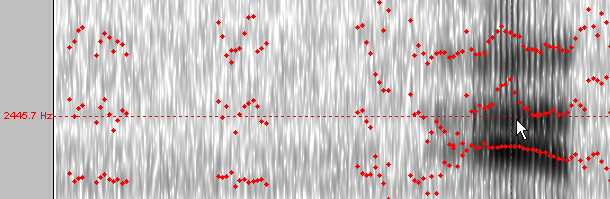
\includegraphics[width=0.8\textwidth]{./figures/PraatSpectrogrGetF1byCursor}
	\end{center}
\end{figure}

\begin{figure}[!tbp]
\caption{\Praat{} -- In case you want to copy and paste your pinpointed Formant value}
\label{step5measure}
	\begin{center}
		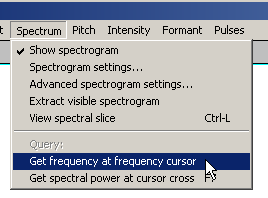
\includegraphics[width=0.8\textwidth]{./figures/PraatSpectrogrGetF1byCursorMenu}
	\end{center}
\end{figure}

If you decide to do that, then you should be consistent across measurements. Choose the same number of points and be explicit about why you decided to take them.  

\subsection{Saving and Plotting the Formant values}

\subsubsection{Saving the values}
Once you get your values, you should start saving them into a spreadsheet. Remember to label the values (figure~\ref{step1save}).

\begin{figure}[!tbp]
\caption{\MSExcel{} -- Saving the Formant values of each recording}
\label{step1save}
	\begin{center}
		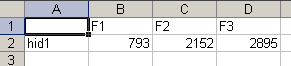
\includegraphics[width=0.8\textwidth]{./figures/Excel1}
	\end{center}
\end{figure}

Once you finished copying the values to the spreadsheet, you will have to average them. In figure~\ref{step2save}, you can see that~\MSExcel{} has a function to do the averaging for you.

\begin{figure}[!tbp]
\caption{\MSExcel{} -- Averaging Formant values. \emph{These values are made up}!}
\label{step2save}
	\begin{center}
		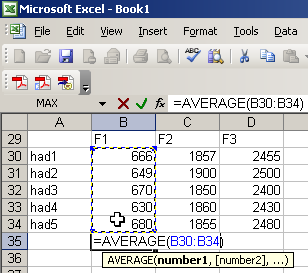
\includegraphics[width=0.8\textwidth]{./figures/Excel3}
	\end{center}
\end{figure}


\subsubsection{Plotting}

Once you have the the average formant values, you are ready to plot your data. You should go to \softmenu{Insert} $>$ \softmenu{Chart} (figure~\ref{step1plot}).

\begin{figure}[!tbp]
\caption{\MSExcel{} -- Creating a chart 1}
\label{step1plot}
	\begin{center}
		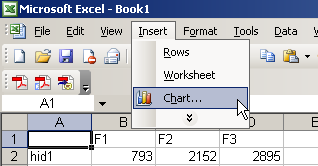
\includegraphics[width=0.8\textwidth]{./figures/Excel2}
	\end{center}
\end{figure}

This will open the \softmenu{Chart Wizard} (figure~\ref{step2plot}). Select \softmenu{XY (Scatter)} in the \softmenu{Chart type} field.

\begin{figure}[!tbp]
\caption{\MSExcel{} -- Creating a chart 2}
\label{step2plot}
	\begin{center}
		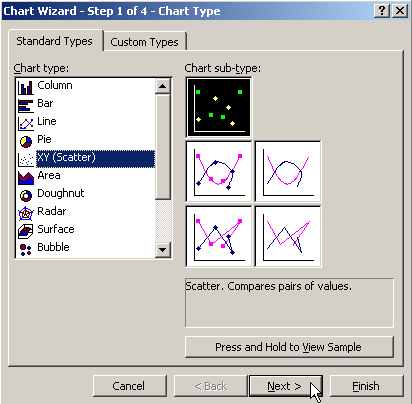
\includegraphics[width=0.8\textwidth]{./figures/ExcelPlot1}
	\end{center}
\end{figure}

Now you have to start entering the data. Every word is going to be its own \softmenu{Series}. Figure~\ref{step3plot} shows (schematically) which value goes where; pay attention to the column names, for instance column A is the word name, B is F1, etc. To keep adding words, just click on the \softmenu{Add} button.

\begin{figure}[!tbp]
\caption{\MSExcel{} -- Creating a chart 3}
\label{step3plot}
	\begin{center}
		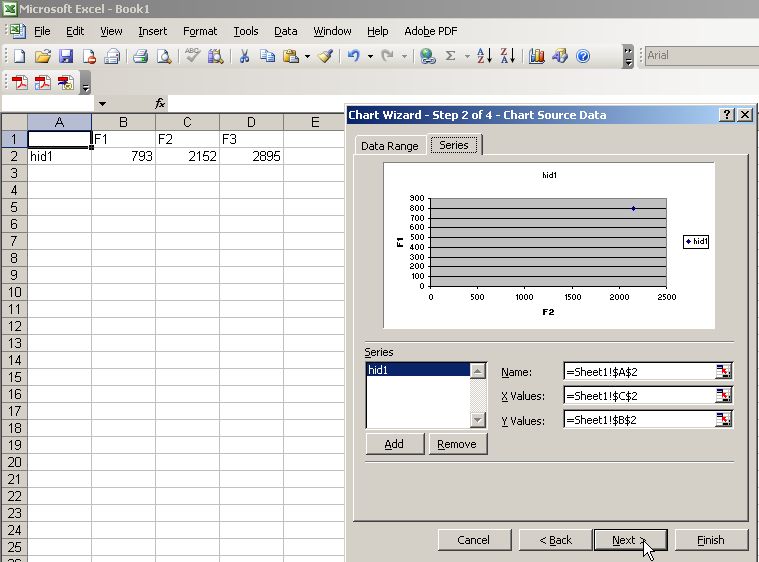
\includegraphics[width=0.8\textwidth]{./figures/ExcelPlot3}
	\end{center}
\end{figure}

Once you entered all the series, you can select a name for your graph. The important thing here is to label the axes appropriately. Remember, F1 is supposed to be the y--axis and F2 is supposed to be the x--axis.

\begin{figure}[!tbp]
\caption{\MSExcel{} -- Creating a chart 4}
\label{step3plot}
	\begin{center}
		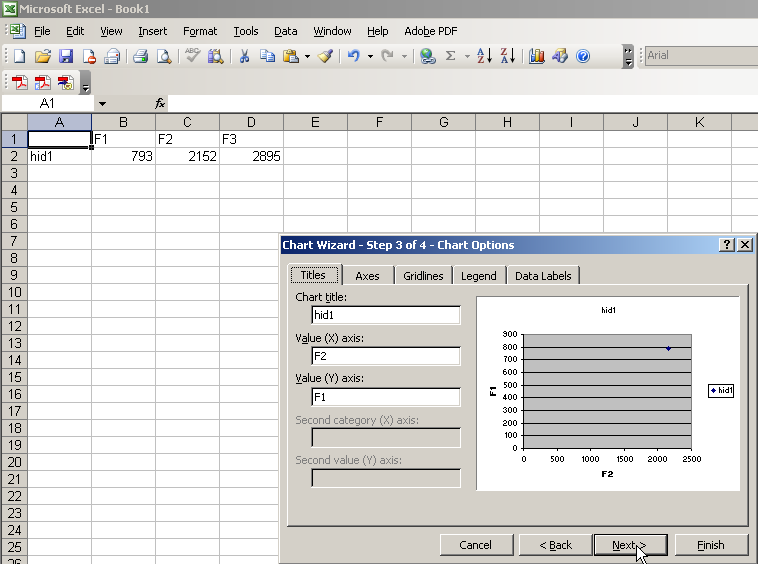
\includegraphics[width=0.8\textwidth]{./figures/ExcelPlot4}
	\end{center}
\end{figure}

Finally, once you have the graph ready, you can label the individual points on it. Put the mouse cursor over the point you want to label (figure~\ref{step4plot}) and double click it. This will open the \softmenu{Format Data Series} window. Check the option \softmenu{Series name} (figure~\ref{step5plot})

\begin{figure}[!tbp]
\caption{\MSExcel{} -- Creating a chart 5}
\label{step4plot}
	\begin{center}
		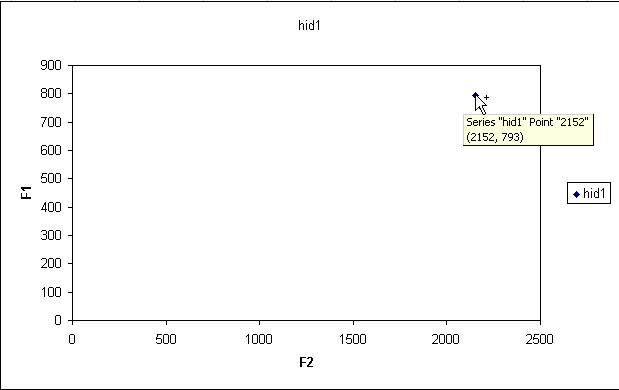
\includegraphics[width=0.8\textwidth]{./figures/ExcelPlot5}
	\end{center}
\end{figure}

\begin{figure}[!tbp]
\caption{\MSExcel{} -- Creating a chart 6}
\label{step5plot}
	\begin{center}
		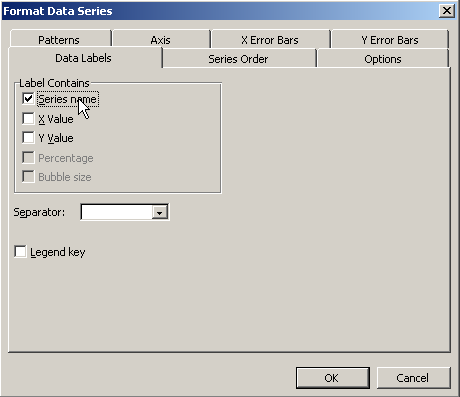
\includegraphics[width=0.8\textwidth]{./figures/ExcelPlot6}
	\end{center}
\end{figure}

\subsubsection{Final plot details}

Now that you know how to plot the vowels in a F1 x F2 space, your final graph should look roughly like figure~\ref{step6plot}\footnote{I only plotted three words for simplicity, your graph should have all of them!}

\begin{figure}[!tbp]
\caption{\MSExcel{} -- Creating a chart 7}
\label{step6plot}
	\begin{center}
		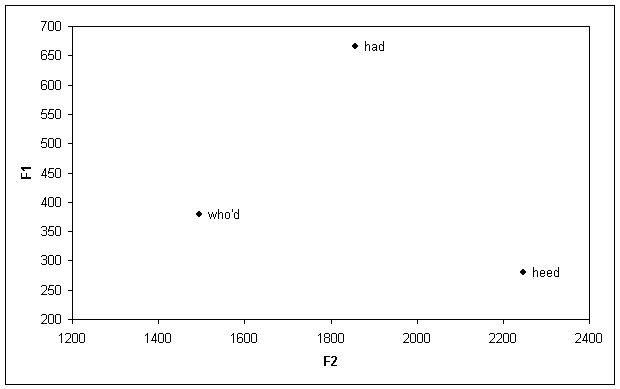
\includegraphics[width=0.8\textwidth]{./figures/ExcelPlot7}
	\end{center}
\end{figure}

I'll leave the prettification details of the graph up to you to figure out, since they are not directly relevant to the lab. I won't deduct any points if your graph is not as pretty as it could be, provided the data is accurately portrayed.

However, plotting a graph is not just about being able to see data, but rather being able to see data \emph{in the most informative way} possible. So you should ask yourself certain questions like \emph{Do I need a legend if the points are labeled?}, \emph{Does the range of the scale on the axes make sense?}, and so on and so forth. This will turn out to be important in the future, so keep that in mind.

\subsection{What you should hand in.}

The second thing I'd like to have is the \MSExcel{} spreadsheet you used to plot your graph. Finally, I'd like a small write up of your efforts. This report should contain the final plot of the average Formant values of each vowel (all in one plot), a small description of how you got them (did you use Praat's formant track function or did you use the mouse cursor?), the problems you encountered and how you overcame them. Try to motivate your decisions during the process. Most importantly, I'd like you to elaborate on the final plot you obtained: Do you see any pattern or suggestive information on it? If so, what is it and what do you think it means?

\subsection{Deadline}

This part of the lab (part (a)) is due by \emph{XXX, FebXXX, at midnight}, via the NYUClasses web interface.

Remember that there are \emph{no penalties} for handing in individual work after the deadline in this class, besides you waiving your right to timely feedback.

However, it was \emph{my fault} that you got the assignment late, and therefore I cannot expect everyone to comply with the deadline. Therefore, for this lab, even if you hand it in late, you will have it back as soon as possible. I apologize for the inconvenience.
